\documentclass{beamer}
\mode<presentation>
\usepackage{hyperref}
\usepackage{pdfpages}
\usepackage{siunitx}
\usepackage{tikz}
\usepackage{xcolor}
\usepackage{physics}
\usepackage{multirow}
\usepackage{graphics}
\usepackage{svg}

\usetikzlibrary{shapes.geometric,angles,quotes,tikzmark}

\definecolor{pGreen}{HTML}{006633}
\definecolor{sgbGreen1}{HTML}{66cc99}
\definecolor{sgbGreen2}{HTML}{ccffcc}

\definecolor{pRed}{HTML}{cc0033}
\definecolor{sgbRed}{HTML}{cc6688}
\definecolor{sgbRed2}{HTML}{FF99CC}

\definecolor{sgbGrey}{HTML}{333333}
\definecolor{sgbGrey2}{HTML}{996666}
\definecolor{sgbGrey3}{HTML}{999966}

\tikzset{3-gon/.pic={
                \draw[fill=sgbGreen1] (0,0) -- (0:3) -- (50:4) -- cycle;
            },
            180deg/.pic={
                \draw[->] (0,0) arc[start angle = 180, end angle=0, radius=5mm] node [left] {$\ang{180}$};
            },
            4-gon/.pic={
                \draw[ultra thick, pRed] (0,0) -- (0:3);
                \draw[ultra thick, pGreen] (0:3) -- (20:4);
                \draw[ultra thick, sgbGrey] (20:4) -- (50:2);
                \draw[ultra thick, sgbGreen1] (50:2) -- (0,0);
            }}

\title{Exploring Modern Mathematics Through the Art of Tiling}
\author[dishajk]{Disha Kuzhively\\ \texttt{disha.jk@icts.res.in}}
\institute{International Centre for Theoretical Sciences - TIFR, Bangalore}
\date[Sci560]{Science Gallery Bangalore}
\begin{document}
\begin{frame}
    \titlepage
\end{frame}
\begin{frame}
    \begin{figure}
        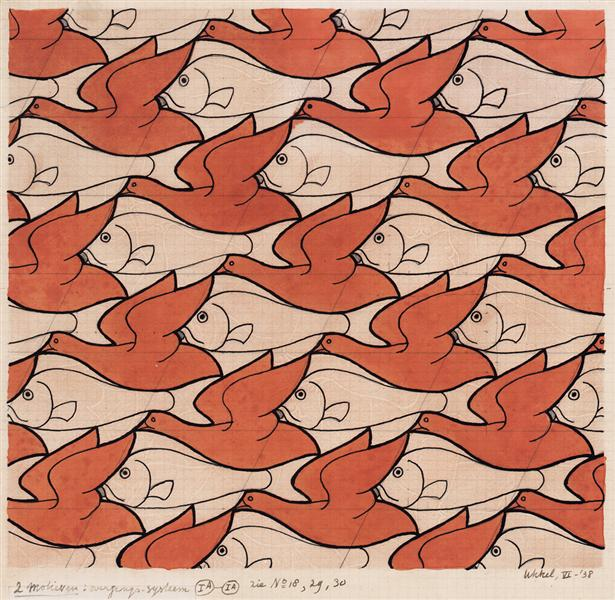
\includegraphics[height=0.8\textheight]{bird-fish}
        \caption{Bird Fish, 1938, MC Escher}    
    \end{figure}
\end{frame}
\begin{frame}
    \begin{figure}
        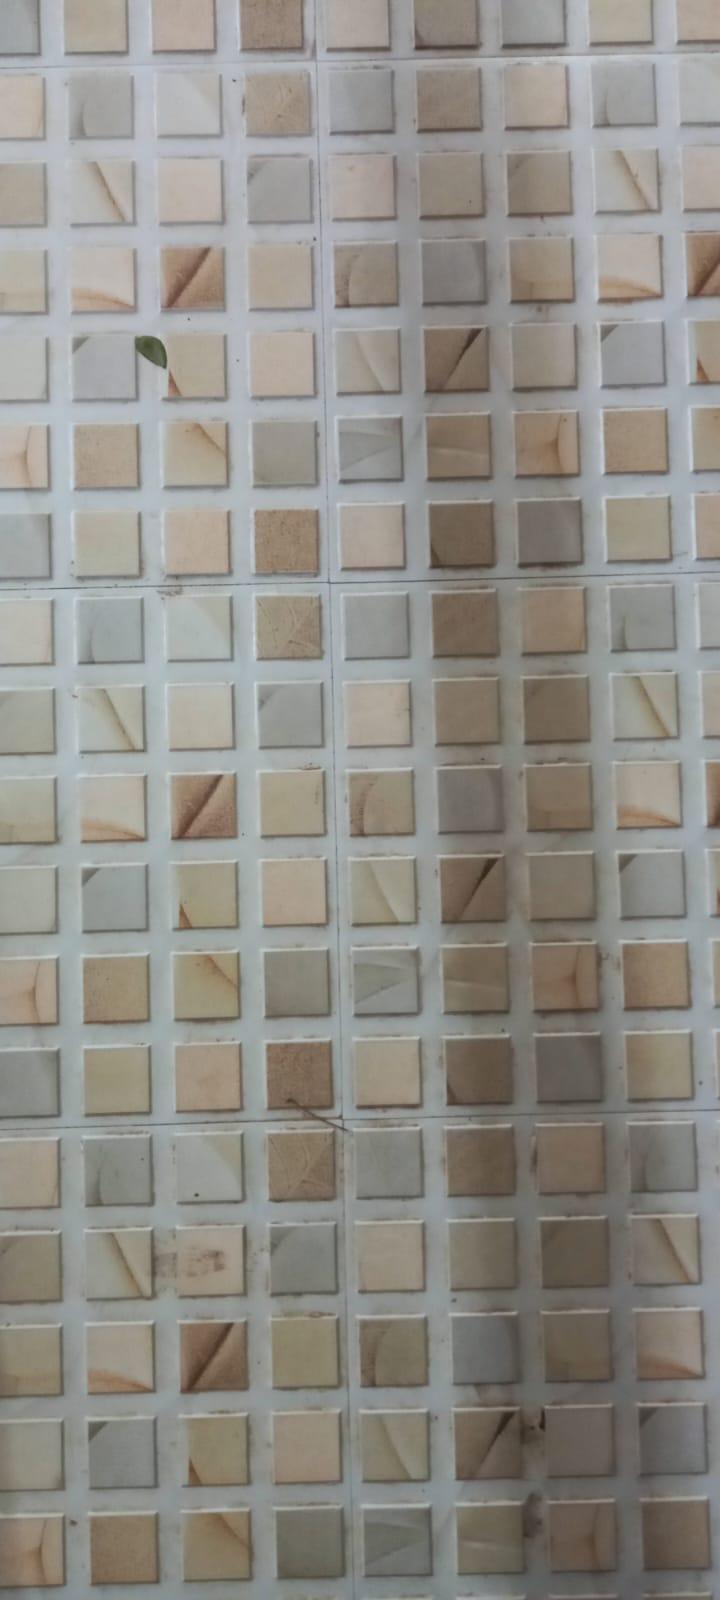
\includegraphics[height=0.5\textheight]{corridor1}
        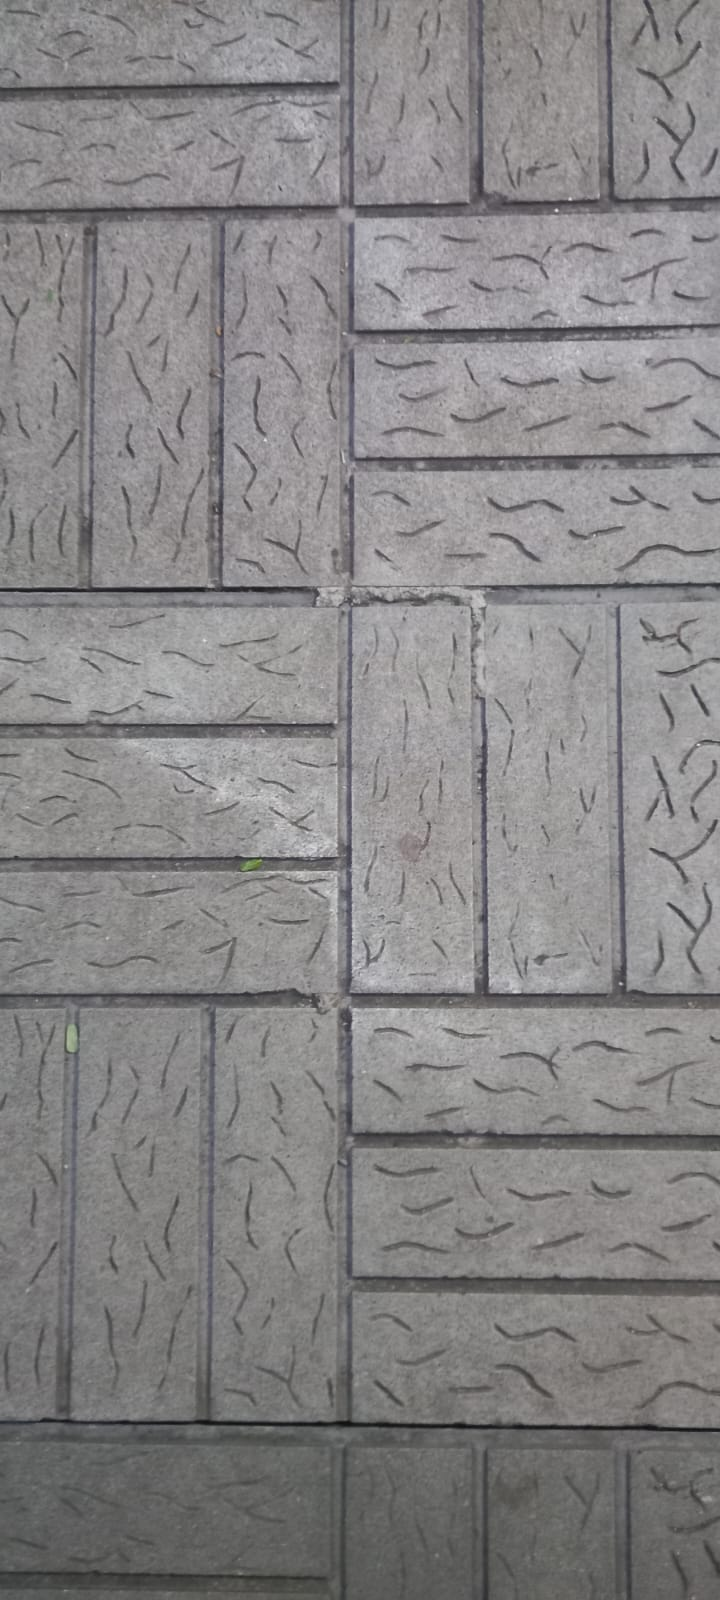
\includegraphics[height=0.5\textheight]{corridor2}
        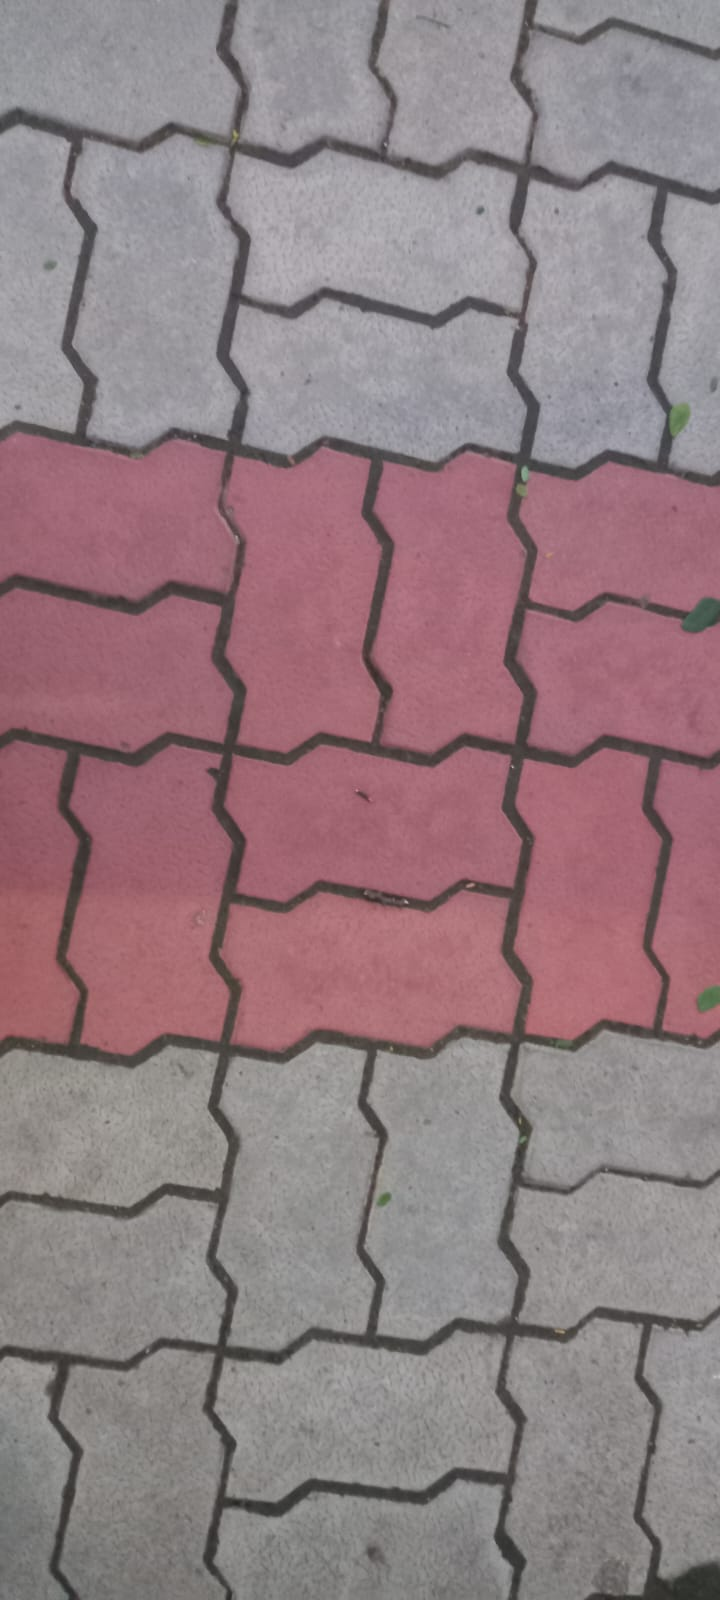
\includegraphics[height=0.5\textheight]{corridor3}
        \caption{Corridors, 2024, Photo: Aysha Mahira}
    \end{figure}
\end{frame}

\begin{frame}
    \begin{figure}
        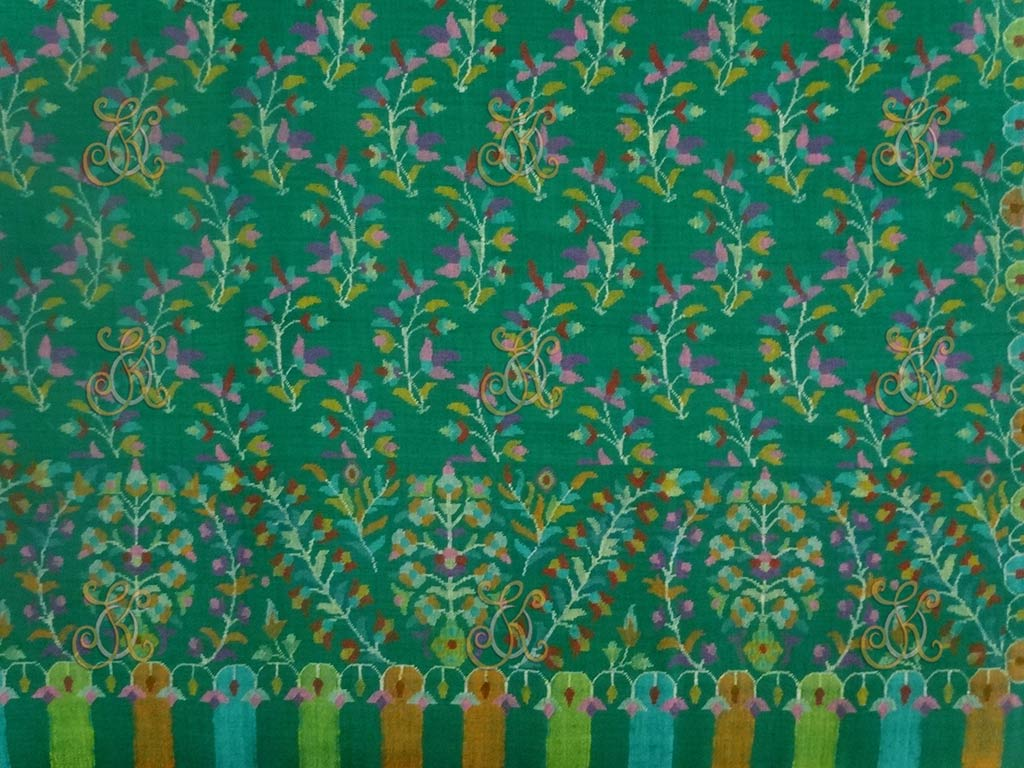
\includegraphics[height=0.7\textheight]{Splendor-of-kashmir-deep-green-kani-pashmina-shawl-by-Varuna-Anand-2}
        \caption{Kani pashmina shawl, Varuna Anand}
    \end{figure}
\end{frame}

\begin{frame}
    \begin{figure}
        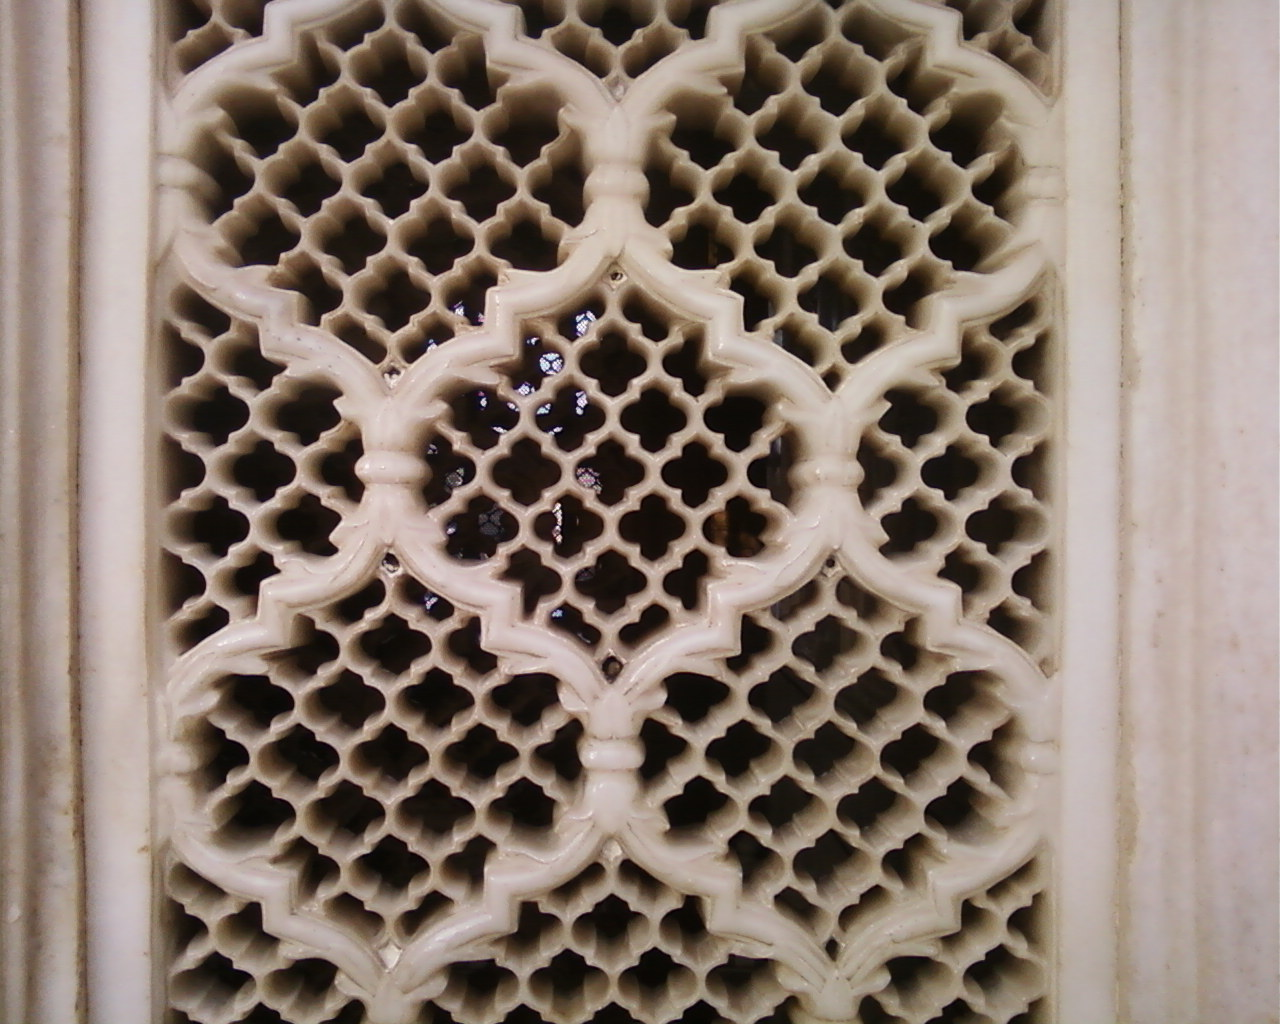
\includegraphics[height=0.7\textheight]{Bibi-Ka-Maqbara-_net}
        \caption{Jali at Bibi Ka Maqbara in Aurangabad. By Niranjan R. Upasani - Own work, CC BY-SA 3.0}
    \end{figure}
\end{frame}

\begin{frame}
    \begin{figure}
        \includegraphics[height=0.7\textheight]{45square}
        \caption{4 - 5 square origami tessellation, pattern from Eric Gjerde, folded by dishajk}
    \end{figure}
\end{frame}

\begin{frame}
\begin{figure}
    \includegraphics[height=0.7\textheight]{Western_honey_bee_on_a_honeycomb}
    \caption{ AWestern honey bee on a honeycomb, Matthew T Rader, \url{https://matthewtrader.com}, CC BY-SA 4.0}
\end{figure}
\end{frame}
\begin{frame}
    \begin{figure}
        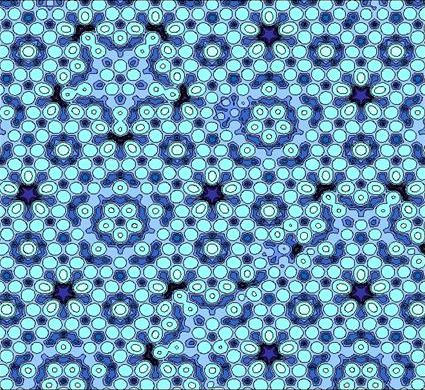
\includegraphics[height=0.5\textheight]{Quasicrystal1}
        \caption{Potential energy surface $\qty(8.6 \times 8.6 nm^2)$ for silver on i-Al-Pd-Mn Quantumcrystal, Physical Review B 75, no. 6 (2007): 064205}
    \end{figure}
    Notice that its \alert{ordered} but \alert{not periodic}!
\end{frame}
\section{What is Tiling?}
\begin{frame}
    \frametitle{Tiling}
    \begin{block}{What is Tiling?}    
    Tiling is the covering of a surface using geometric shapes while ensuring there are \alert{no overlaps} and \alert{no gaps}.
    \end{block}  
\end{frame}
\begin{frame}
    \frametitle{Tiling with Convex Regular Polygons}
    \only<1>{A convex regular polygon has $n$ straight edges and $n$ equal internal angles. It is convex because any line segment joining two vertices passes entirely through the polygon's interior.}
    
    \only<2>{Can you tile with convex regular polygons?} 
    
    \only<3-4,11-13>{How many \alert{edge to edge} tilings are possible using \alert{only one} type of tile?}

    \only<14->{How many \alert{edge to edge} tilings are possible using \alert{more than one} type of tile?}

    \only<1-3>{\tikz {\foreach \a in {3,...,6}{
        \node[regular polygon, regular polygon sides=\a, fill=sgbGreen2, draw, minimum size=2.25cm] at (\a*2.25,0) {};
        \node[regular polygon, regular polygon sides={\a+3}, draw, fill=sgbGreen2, minimum size=2.25cm] at (\a*2.25,-2.5) {};
        }}}
    
    \only<4>{
        \begin{columns}
            \begin{column}{0.4\textwidth}
                \begin{figure}
                \includesvg[scale=0.25]{Academ_Periodic_tiling_by_squares_of_two_different_sizes}
                \caption{Non edge to edge tiling, in this case a Pythagorean tiling. By Arthur Baelde}
                \end{figure}
            \end{column}
            \begin{column}{0.4\textwidth}
                \begin{figure}
                    \includesvg[scale=0.45]{Tiling_snub_3-6_left_simple}
                    \caption{Edge to edge tiling}
                \end{figure}
            \end{column}
        \end{columns}
        \tikz \node[draw] at (0,0) {edge to edge tiling example};
        \tikz \node[draw] at (0,0) {not edge to edge tiling example};}
    
    \only<5-10>{Internal angle of an $n$-sided polygon}
    
    \only<19-21>{Consider $m=3$}
    
    \only<22>{
        Archimedean tilings
        
        \begin{tabular}{ l|l|l|l|l|l }
            $m$ & $n_1$ & $n_2$ & $n_3$ & $n_4$ & $n_5$ \\\hline
            \multirow{3}{2em}{3}& 3 & 12 & 12 & & \\  
            &4 & 6 & 12 & & \\
            &4 & 8 & 8 & &\\ \hline
            \multirow{3}{2em}{4} & 3 & 6 & 3 & 6 & \\
            & 3 & 4 & 6 & 4 & \\\hline
            \multirow{3}{2em}{5} &3 & 3 & 4 & 3 & 4\\
            &3 & 3 & 3 & 4 & 4\\
            & 3 & 3 & 3 & 3 & 6
           \end{tabular}
    }
    \begin{columns}
        \begin{column}{0.4\textwidth}
            \only<5>{
                \tikz \node[regular polygon, regular polygon sides={11}, draw=sgbRed, minimum size=5cm] at (0,0) {11-gon};
            }

            \only<6>{
                \tikz {\node[regular polygon, regular polygon sides={11}, draw=sgbRed, minimum size=5cm] at (0,0) {};
                \foreach \angle in {0,...,10}{
                \draw (0,0) -- ({90+\angle*360/11}:2.5);}
                }
            }

            \only<7>{
                \tikz{\node[regular polygon, regular polygon sides={11}, draw=sgbRed, minimum size=5cm] at (0,0) {};
                \foreach \angle in {0,...,10}{
                    \draw (0,0) -- ({90+\angle*360/11}:2.5);
                    }
                \filldraw[fill=sgbGreen2,draw=black] (0,0) -- (90:0.25) arc [start angle=90,end angle={90+360/11},radius=0.25];
                \filldraw[fill=sgbGreen2,draw=black] (90:2.5) -- (90:2.25) arc [start angle=270,end angle={270-9*90/11},radius=0.25];
                \filldraw[fill=sgbGreen2,draw=black] ({90+360/11}:2.5) -- ({90+360/11}:2.25) arc [start angle={270+360/11},end angle={270++360/11+9*90/11},radius=0.25];
                }}

            \only<8>{
                \tikz{\node[regular polygon, regular polygon sides={11}, draw=sgbRed, minimum size=5cm] at (0,0) {};
                \foreach \angle in {0,...,10}{
                    \draw (0,0) -- ({90+\angle*360/11}:2.5);
                    }
                \filldraw[fill=sgbGreen2,draw=black] (0,0) -- (90:0.25) arc [start angle=90,end angle=450,radius=0.25];
                \foreach \angle in {0,...,10}{
                \filldraw[fill=sgbGreen2,draw=black] ({90+\angle*360/11}:2.5) -- ({90+\angle*360/11}:2.25) arc [start angle={270+\angle*360/11},end angle={270+\angle*360/11-9*90/11},radius=0.25];
                \filldraw[fill=sgbGreen2,draw=black] ({90+360/11+\angle*360/11}:2.5) -- ({90+360/11+\angle*360/11}:2.25) arc [start angle={270+\angle*360/11+360/11},end angle={270+\angle*360/11+360/11+9*90/11},radius=0.25];}}
                }
            
            \only<9>{
                \tikz{\node[regular polygon, regular polygon sides={11}, draw=sgbRed, minimum size=5cm] at (0,0) {};
                \foreach \angle in {0,...,10}{
                    \draw (0,0) -- ({90+\angle*360/11}:2.5);
                }
                \foreach \angle in {0,...,10}{
                    \filldraw[fill=sgbGreen2,draw=black] ({90+\angle*360/11}:2.5) -- ({90+\angle*360/11}:2.25) arc [start angle={270+\angle*360/11},end angle={270+\angle*360/11-9*90/11},radius=0.25];
                    \filldraw[fill=sgbGreen2,draw=black] ({90+360/11+\angle*360/11}:2.5) -- ({90+360/11+\angle*360/11}:2.25) arc [start angle={270+\angle*360/11+360/11},end angle={270+\angle*360/11+360/11+9*90/11},radius=0.25];
                    }}}
        
            \only<10>{
                \tikz{\node[regular polygon, regular polygon sides={15}, draw=sgbRed, minimum size=5cm] at (0,0) {$n$-gon};
                }}
    
            \only<11-12>{
                \tikz{\foreach \angle in {0,...,4}{
                        \draw (0,0) -- ({90+\angle*360/5}:2.5);}
                    \foreach \angle[count=\ai] in {0,...,2}{
                        \draw (0,0) ++ ({70+\angle*360/5}:2) node[left] {\ai};}
                        \draw (0,0) ++ ({70+3*360/5}:2) node[left] {$\ldots$};
                        \draw (0,0) ++ ({70+4*360/5}:2) node[left] {$m$};
                        }}
            \only<13>{
                \tikz{
                    \clip (0.1,0.1) rectangle (2.5,2.5);
                    \foreach \row in {0,...,3}{
                        \draw (0,{\row*sqrt(3)/2}) --++ (0:3);
                        \draw (\row,0) --++ (60:4);
                        \draw (\row,0) --++ (120:4);}}
                \tikz{
                \clip (0.1,0.1) rectangle (2.5,2.5);
                \draw (0,0) grid (3,3);}
                }
        
            \only<15-18>{
                \tikz{
                    \foreach \angle in {7, 15, 22, 29, 34}{
                        \draw (0,0) -- ({10*\angle}:2);
                    }
                    \foreach \angle[count=\ai] in {7, 15, 22}{
                        \node at ({10*\angle+20}:2) {$n_\ai$-gon};
                    }
                    \node[left] at ({10*29+20}:2) {\ldots};
                    \node[left] at ({10*34+20}:2) {$n_m$-gon};
                }
            }
            \only<20>{
                \begin{center}
                    \begin{tabular}{ l|l|l }
                     $n_1$ & $n_2$ & $n_3$ \\\hline 
                     3 & 12 & 12 \\  
                     4 & 6 & 12 \\
                     4 & 8 & 8 \\
                     3 & 7 &42 \\
                     3 & 8 &24 \\
                     3 & 9 &18 \\
                     3 & 10 &15 \\
                     4 & 5 &20 \\
                     5 & 5 &10 
                    \end{tabular}
                \end{center}
            }
            \only<21>{
                \begin{center}
                    \begin{tabular}{ l|l|l }
                     $n_1$ & $n_2$ & $n_3$ \\\hline 
                     3 & 12 & 12 \\  
                     4 & 6 & 12 \\
                     4 & 8 & 8 \\
                     \tikzmark{start}3 & 7 &42 \\
                     3 & 8 &24 \\
                     3 & 9 &18 \\
                     3 & 10 &15 \\
                     4 & 5 &20 \\
                     5 & 5 &10\tikzmark{end} 
                    \end{tabular}
                    \tikz[remember picture]\draw[overlay] ([yshift=.35em]pic cs:start) -- ([yshift=.35em]pic cs:end);
                \end{center}
            }
        \end{column}
        \begin{column}{0.6\textwidth}
            \only<6-9>{for $n$ = 11, we have 11 triangles.}
            
            \only<7-10>{Sum of angles of one triangle = $\pi$
            
            $\pi = \ang{180}$}
            
            \only<8-9>{Sum of angles of 11 triangles = $11\pi$}
            
            \only<9>{Sum of internal angles = $11\pi - 2\pi$
            
            Each internal angle  = $\flatfrac{\qty(11\pi - 2\pi)}{11}$}
            
            \only<10>{when we have $n$ triangles,

            Sum of angles of $n$ triangles = $n\pi$

            Sum of internal angles = $n\pi - 2\pi$}
            
            \only<10-12,16-18>{
                Internal angle  = $\flatfrac{\qty(n - 2)\pi}{n} = A_n$
            }
            
            \only<11-12>{
                $m \times A_n = \ang{360} = 2\pi$
            }
            
            \only<13>{
                \tikzset{cell/.pic={
                \draw (0,{sqrt(3)/4})--++(0:0.25) --++(60:0.5)--++(0:0.5)--++(300:0.5)--++(0:0.25);
                \draw (0.25,{sqrt(3)/4})--++(300:0.5);
                \draw (1.25,{sqrt(3)/4})--++(240:0.5);
            }}
            \tikz{
            \clip (0.1,0.1) rectangle (4,3);
            \foreach \x in {0,...,3}{
                \foreach \y in {0,...,3}{
                    \draw ({1.5*\x},{\y*sqrt(3)/2}) pic {cell};
                }};}
            }
            
            \only<12-13>{
                \begin{equation*}
                \frac{1}{m} + \frac{1}{n} = \frac{1}{2}
                \end{equation*}
            }
            \only<16-18>{
                \begin{equation*}
                    A_{n_1}+A_{n_2}+A_{n_3}+\ldots+A_{n_m} = 2\pi
                \end{equation*}
            }
            \only<17-21>{
                \begin{equation*}
                    \frac{m}{2} - \qty(\frac{1}{n_1}+\frac{1}{n_2}+\frac{1}{n_3}+\ldots+\frac{1}{n_m})=1
                \end{equation*}
            }
            \only<19-21>{
                \begin{equation*}
                    \frac{3}{2} - \qty(\frac{1}{n_1}+\frac{1}{n_2}+\frac{1}{n_3})=1
                \end{equation*}
            }
        \end{column}
    \end{columns}    
\end{frame}

\begin{frame}
    \frametitle{Tiling with Convex non-Regular Polygons}
    \only<1>{\begin{itemize}
    % \item Convex polygons of more than six sides \alert{cannot} tile the plane.\footnote{Can be showed using Euler's Formula}

    \item Let's look at tilings using polygons of sides 3 (triangles), 4 (quadrilaterals), 5 (pentagons), and 6 (hexagons)
    \end{itemize}}

    \only<2-4>{1. Tiling with non equilateral triangles}

    \only<2-3>{
        \tikz {\draw (0,0) pic {3-gon};
        }
    }
    \only<3>{
        \tikz {\draw (3.5,{2*sin(59)}) pic {180deg};
        \draw (8,{4*sin(50)}) pic[rotate=180] {3-gon};
        }
    
        Parallelogram
    }

    \only<4>{
        \tikz {
            \foreach \x in {0,1,2}{
                \foreach \y in {0,1}{
                    \draw ({\x*3},{4*sin(50)*\y}) pic {3-gon};
                    \draw ({\x*3+4*cos(50)},{(\y+1)*4*sin(50)}) pic[rotate=180] {3-gon};
                }
            }
        }
    }
    \only<5-7>{2. Tiling with quadrilaterals (4 sided figures)}
    \only<5-6>{
        \tikz{\draw (0,0) pic {4-gon};
        }
    }
    \only<6>{
        \tikz {\draw (0,0) pic {180deg};
        \draw ({1.75+4*cos(20)},{2*sin(50)}) pic[rotate=180] {4-gon};
        }
    }
    \only<7>{
        \tikz{
            \foreach \x in {0}{
                \foreach \y in {0}{
                    \draw (\x,\y) pic {4-gon};
                    \draw ({\x+3},\y) pic[rotate=180] {4-gon};
        }}}
        Hexagon with equal and parallel opposite edges
    }
    \only<8>{3. Tiling with pentagons
    
    }
    \only<9>{4. Tiling with hexagons (1918, Reinhardt)
    
    }
    \only<10>{Conway Criterion}
    \only<11>{Domino tiling}
\end{frame}
\begin{frame}
    Break 1
\end{frame}
\begin{frame}
    \frametitle{Periodic vs. non-priodic}
    \begin{itemize}
        \item<1-4> In peiodic tiling, one can define a region as a 'unit cell' and the unit cell can then be used to tile the plane by translation alone - i.e. without rotating or reflecting it.
        \item<2-4> Some shapes can tile only periodically - e.g. regular hexagon
        \item<3-4> Some shapes can be tiled in both ways - e.g. isoceles triangles - Central tessellations
        \item<4-> Are there shapes that can tile \alert{only} non-periodically?
    \end{itemize}
\end{frame}
\begin{frame}
    \frametitle{Wang's Conjecture}

    Wang's conjecture states that if a set of tiles can tile the plane, then they can always be arranged to do so periodically (Wang 1961)

    Such tiling will have a decision procedure relating this to decision questions in symbolic logic
    \only<2>{

    Wang's conjecture was falsified in 1964 by R Berger by constructing a set of 20,426 tiles that tiles only periodically. He later reduced this to 104.

    D Knuth brought this number down to 92.

    Ultimately Penrose proposed a set 6 non-square tiles using which one can tile non-periodically.}
    \only<1>{
        \includesvg{WangsConjecture11Tiling_1000}
    }
\end{frame}
\begin{frame}    
\frametitle{Penrose Tiles}
\begin{columns}
    \begin{column}{0.45\textwidth}    
    \includesvg[scale=0.3]{penrose-kite-single}
Kite    
\end{column}
    \begin{column}{0.45\textwidth}    
            \includesvg[scale=0.3]{penrose-dart-single}
        Dart
    \end{column}
\end{columns}
\end{frame}
\begin{frame}    
    \frametitle{Penrose Tiles}
    \begin{columns}
        \begin{column}{0.45\textwidth}    
                \includesvg[scale=0.15]{penrose-kite-single}
            Kite
        \end{column}
        \begin{column}{0.45\textwidth}    
                \includesvg[scale=0.15]{penrose-dart-single}
            Dart
        \end{column}
    \end{columns}
    \vspace{2cm}

        \only<1>{Task 1: Study the angles.} 
        \only<2>{Task 2: Tiling. To force aperiodicity, ensure that abutting edges join same type of arcs (either dashed or dotted).}
        \only<3>{Task 3: What's the ratio of kites and darts?}
        \only<4>{Task 4: Symmetry?}
        \only<5>{Task 5: Prove that the number of Penrose tilings is uncountable.}

        \only<6->{Homework: Colorability, Ammann bars}

    \end{frame}
    \begin{frame}    
Break 2
    
    \end{frame}
    \begin{frame}
    \frametitle{The ein - stein problem}
    \only<1-2>{Is there a \alert{single} tile that will tile the plane only aperiodically?}

    \only<2>{
        In March 2023, David Smith (amateur mathematician and retired print technician), Craig S. Kaplan (computer scientist and mathematician),  Joseph Samuel Myers (software developer), and Chaim Goodman-Strauss (mathematician) showed that the hat tile can be used to tile aperiodically
        \begin{figure}
        \includesvg[scale=0.35]{Smith_aperiodic_monotiling}
        \caption{An aperiodic tiling using the hat tile by Smith, Myers, Kaplan and Goodman-Strauss, redrawn by Gringer. Note that the hat tile's mirror image is also considered}
    \end{figure}
    }
    \only<3>{\begin{figure}
        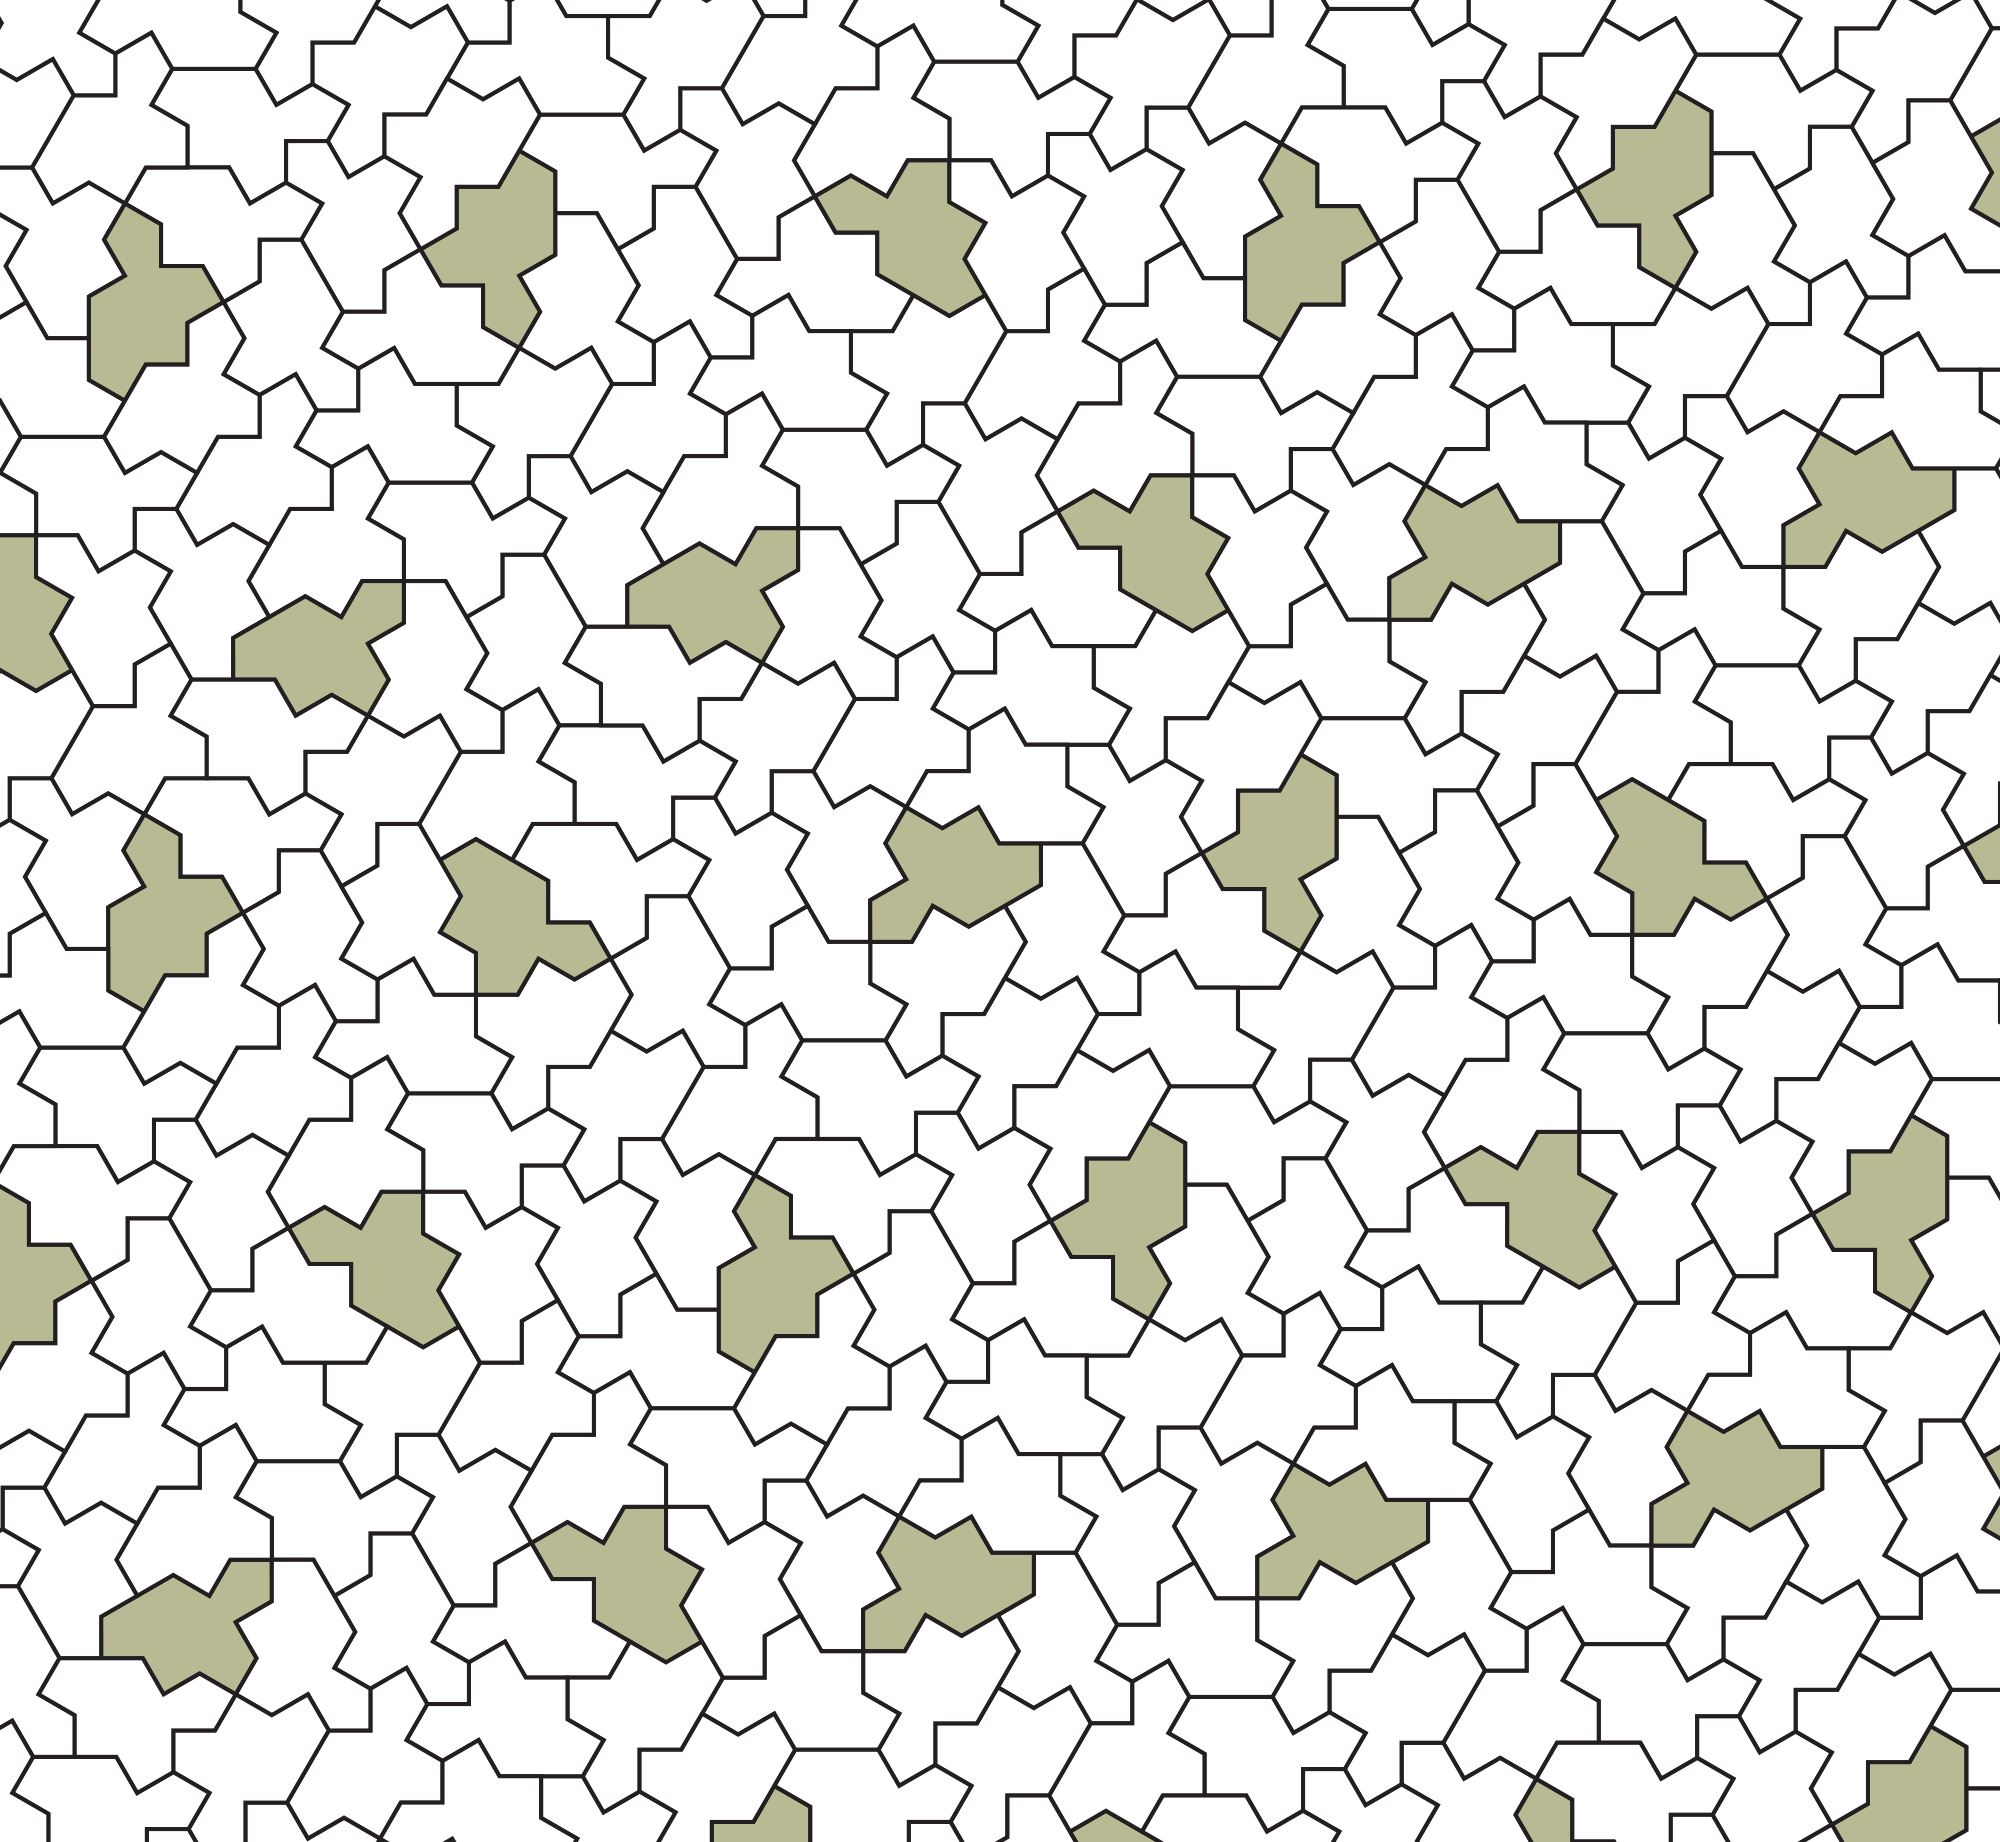
\includegraphics[height=0.7\textheight]{Aperiodic_monotile_tiling.png}
        \caption{Aperiodic tiling with "Tile(1,1)" using only rotations and translations. David Smith, Joseph Samuel Myers, Craig S. Kaplan, and Chaim Goodman-Strauss, 2023}
    \end{figure}}
\end{frame}

\begin{frame}
    \frametitle{Reference}
    \begin{enumerate}
        \item \url{https://cs.uwaterloo.ca/~csk/spectre/}
        \item Smith, David, et al. "An aperiodic monotile." arXiv preprint arXiv:2303.10798 (2023).
        \item Gardner, Martin. Penrose tiles to trapdoor ciphers: And the return of Dr Matrix. Cambridge University Press, 1997.
        \item Smith, David, et al. "A chiral aperiodic monotile." arXiv preprint arXiv:2305.17743 (2023).
    \end{enumerate}
\end{frame}
\begin{frame}
    \frametitle{Acknoledgements, Ad break, and Questions}
    \begin{enumerate}
        \item \url{icts.res.in/outreach}
        \item Maths Circle India
        \item MathSpark
        \item PrISM
        \item Public Lectures at ICTS 
        \item Einstein Lectures
        \item Write to \url{outreach@icts.res.in} or \url{disha.jk@icts.res.in}
    \end{enumerate}
    \vspace{0.5cm}
    Thanks to Roshini, Anugraha, Sam, Rajarshi, Ruby, Javed, Anjana, and Anika 
\end{frame}
\end{document}    


\begin{frame}
Escher's ascending descending - penrose staircases
\end{frame}
\begin{frame}
Ratio of number of darts and kites
if the ratio was rational? - periodic Tiling
place the forced pieces first
when you have choices - one can lead to a point where no more pieces can be legally added
number of penrose tilings? - 'uncountable'
uncountable meaning? - e.g. rational numbers are countable, real numbers are uncountable

\end{frame}


